\documentclass[12pt,a4paper]{report}
\usepackage{amsmath,amsthm,amssymb,mathrsfs,graphicx,comment,blindtext,subfiles,tikz}
\usepackage[noend]{algorithmic} %algorithmic environment
\usetikzlibrary{shapes.geometric,calc}
\allowdisplaybreaks


\newtheorem{theorem}{Theorem}[section]
\newtheorem{definition}[theorem]{Definition}
\newtheorem{example}[theorem]{Example}
\newtheorem{corollary}[theorem]{Corollary}
\newtheorem{lemma}[theorem]{Lemma}
\newtheorem{proposition}[theorem]{Proposition}
\newtheorem{remark}[theorem]{Remark}
\newtheorem{algorithm}[theorem]{Algorithm}

\renewcommand{\baselinestretch}{1.5}
\renewcommand{\algorithmicrequire}{\textbf{Input:}}
\renewcommand{\algorithmicensure}{\textbf{Output:}}

%% Replace init/inif with \initial or "in"
\DeclareMathOperator{\initial}{in}

\begin{document}

\chapter{Groebner Walks and Variations}
With the initial groundwork out of the way, we can begin to outline the Groebner Walk and explore variations and improvements of this. 

\section{Extra Preparation}
We can find a single Groebner cone by Buchberger's algorithm and Corollary 3.1.10 (from \cite{AndersPHD}) for some term order. Since we have shown that the graph of the Groebner fan of I is connected, we can pick and choose any graph traversal algorithm we want to compute the full dimensional Groebner cones. To do this, we need to be able to find edges (or connecting facets) and we need to find neighbours along an edge.

Throughout the graph enumeration process, we can represent Groebner cones by their marked reduced Groebner bases instead of any other of their qualities such as their inequalities, term orders etc.. The reasoning for doing this is due to the following theorem (which we will take without proof):

\begin{theorem}
Let $I \subseteq R = K[x_{1}, \cdots, x_{n}]$ be an ideal. The marked reduced Groebner bases of I, the monomial initial ideals of I (w.r.t positive vectors), and the full-dimensional Groebner cones are in bijection.
\end{theorem}

\section{Local Change}
%Reference to link is clumsy here?
Let $G_{\prec} (I)$ be some marked Groebner basis and F be a flippable facet of $C_{\prec} (I)$. We let Flip$(G_{\prec} (I), F)$ denote the unique reduced Groebner basis different from $G_{\prec} (I)$ whose Groebner cone also has F as a facet. We describe an algorithm for computing this, given $G_{\prec} (I)$ and an inner normal vector $link(C_{-< (I)}, v) $($ = w \in \mathbb{R^n}, v + \epsilon w \in C_{-< (I)}$, for $\epsilon > 0$ sufficiently small). We will denote this as $Link(v)$

For a marked Groebner basis $G$ and a polynomial f, we let $f^{G}$ denote the normal form of $f$ mod $G$. This normal form only depends on the markings of $G$.

%Polynomial is a terrible name for an algorithm, but what else do I call it??
We will now introduce algorithm components consisting of the Polynomial, the Lifting and the Flipping algorithms. Proof of all these algorithms can be found at \cite{AndersPHD}.

\begin{algorithm}[Polynomial]\
 \begin{algorithmic}[1]
    \REQUIRE{A marked reduced Groebner basis $G_{\prec} (I)$, v-homogeneous polynomial $g \in \initial_{v} (I)$ where v is some vector in $C_{\prec}(I)$.}
    \ENSURE{A polynomial $f \in I$ where $\initial_{v}(f) = g$.}
    \RETURN{$f := g - g^{G_{\prec} (I)}$;}
\end{algorithmic}
\end{algorithm}

\begin{algorithm}[Lifting]\
 \begin{algorithmic}[1]
    \REQUIRE{Marked reduced Groebner bases $G_{\prec} (I), G_{{\prec '}_{v}}(\initial_{v} (I))$, where $v \in C_{\prec} (I)$ is some vector, $\prec$ and ${\prec '}$ are some term orders. Here, either I must be homogeneous, or $v \in \mathbb{R}_{\geq 0} ^{n}$.}
    \ENSURE{The marked reduced Groebner basis $G = G_{{\prec '}_{v}} (I)$.}
    \STATE $G := \{g - g^{G_{\prec} (I)} : g \in G_{{\prec '}_{v}} (\initial_{v} (I)) \}$;
    \STATE Mark term $\initial_{{\prec '}_{v}} (g)$ in each element $g - g^{G_{\prec} (I)}$ in $G$;
    \STATE Turn the minimal basis $G$ into a reduced basis;
    \RETURN{Marked reduced Groebner basis G}
\end{algorithmic}
\end{algorithm}

%%Do I need to return anything?? for this algorithm?
\begin{algorithm}[Flipping]\
 \begin{algorithmic}[1]
    \REQUIRE{A marked reduced Groebner basis $G_{\prec} (I)$ with $\prec$ some term order, inner normal vector $\alpha$ of a flippable facet $F$ of $C_{\prec} (I)$.}
    \ENSURE{$G = flip(G_{\prec} (I), F)$.}
    \STATE Let $v$ be a positive vector, in relative interior of $F$;
    \STATE Compute $G_{\prec} (\initial_{v} (I)) = \{\initial_{v} (g): g \in G_{\prec} (I)$ \};
    \STATE Compute marked basis $G_{\prec - Link(v)} (\initial_{v} (I))$ from $G_{\prec} (\initial_{v} (I))$ using Buchberger's Algorithm;
    \STATE Compute $G := G_{{\prec - Link(v)}_{v}}$ (I) from $G_{\prec} (I)$ and $G_{\prec - Link(v)} (\initial_{v} (I))$ using Algorithm 4.2.2 above;
    \RETURN{PLACEHOLDER}
\end{algorithmic}
\end{algorithm}


In the "special" case where $F$ is a facet, we can state the following: A term of g is in $\initial_{v} (g)$ if and only if its exponent vector minus exponent of $\initial_{\prec} (g)$ parallel to $Link(v)$. The term order $\prec$, nor does the vector v, needs to be known during the entirety of this computation.


\section{The Straight Line Walk}
Here, we will use Chapter 3 of \cite{GenericGroebner} as a basis for the rest of the chapter.

In general, the very basis of the Groebner Walk is the movement from one Groebner cone to another, in order to convert a Groebner Basis from one term order to another. There are multiple ways to achieve this and so there are multiple variations on the Groebner Walk. We will first describe the basic algorithm underpinning the Groebner Walk, The Straight Line Walk before moving onto potential variations. 

To begin, let $\prec_{1}, \prec_{2}$ be two term orders and $I$ an ideal in $R$. Suppose we know the reduced Groebner basis $G$ for $I$ over $\prec_{1}$. If $w \in C_{\prec_{1}} (I) \cap C_{\prec_{2}} (I)$ lies on the common face of the two Groebner cones, then $G_{w} = \{ \initial_{w} (g) \vert g \in G \}$ is the reduced Groebner basis for $\initial_{w} (I)$ over $\prec$. Now we need to perform a lifting of $G_{W}$ to a Groebner basis for I over $\prec_{2}$ is required. It involved a Groebner basis computation for $\initial_{w} (I)$ over $prec_{2}$. The point of performing this computation is the fact that if $F = C_{\prec_{1}} (I) \cap C_{\prec_{2}} (I)$ is a high dimensional face (i.e. a facet) and $w$ is in the relative interior of $F$, the ideal $\initial_{w} (I)$ is close to a monomial ideal and this Groebner basis computation becomes very easy.

Given a term order $\prec$ and a vector $w \in \mathbb{R}^{n} _{\geq 0}$, we define the new term order $\prec_{w}$ by $u \prec_{w} v$ if and only if $\langle u, w \rangle < \langle v, w \rangle$, or $\langle u, w \rangle = \langle v, w \rangle$ and $u \prec v$.

%%Is this too much repetition? Probably? 
We will recall the following from \cite{GenericGroebner}

Firstly, for an ideal $I \subseteq R$ and $w \in \mathbb{R}_{\geq 0}^{n}$, we have:
\begin{equation*}
    \initial_{{\prec} ( \initial_{w}} (I)) = \initial_{{\prec}_{w}} (I)
\end{equation*}

%%This has all been clarified by algorithms above?
Secondly, let $I \subseteq R$ be an ideal and have two term orders, $\prec_{1}, \prec_{2} on R$. Suppose G is reduced Groebner basis for I over $\prec_{1}$. If $w \in C_{\prec_{1}} (I) \cap C_{\prec_{2}} (I)$, then:

\begin{itemize}
    \item The reduced Groebner basis for $\initial_{w}$ over $\prec_{1}$ is $G_{w} = \{ \initial_{w} (g) | g \in G\}$.
    \item If H is the reduced Groebner basis for $\initial_{w} (I)$ over $\prec_{2}$, then $\{ f - f^{G} | f \in H \}$ is a minimal Groebner basis for I over $\prec_{2w}$. $f^{G}$ is remainder obtained by dividing f modulo G.
    \item The reduced Groebner basis for I over $\prec_{2w}$ coincides with the reduced Groebner basis for I over $\prec_{2}$.
\end{itemize}

We now can outline the Groebner Walk, by sketching a single step of the algorithm. Subsequent steps of the algorithm follow from this single step outline. Suppose $w_{0} \in C_{{\prec}_{1}} (I), \tau_{0} \in C_{{\prec}_{2}} (I)$, and G is the reduced Groebner basis for I over $\prec_{1}$. Here we consider term orders $\prec_{1}$, $\prec_{2}$ to be rational, given by $w = (w_{1}, \cdots w_{n})$, $\tau = (\tau_{1}, \cdots \tau_{n})$. Now consider the line:
\begin{equation*}
    w(t) = (1-t)w_{0} + t \tau_{0}, 0 \leq t \leq 1
\end{equation*}
in the Groebner fan of I from $w_{0}$ to $\tau_{0}$. We know the reduced Groebner basis at $w(0) = w_{0}$ (being G). Consider the "last" $w^{'} = w(t^{'})$ in $C_{{\prec}_{1}} (I) = C_{{\prec}_{1}} (G)$. We want $t^{'}$ to satisfy:
%%Turn into a list

\begin{enumerate}
    \item $0 \leq t^{'} \leq 1$.
    \item $w(t) \in C_{\prec}_{1} (I)$ for $t \in [0, t^{'}] $and$ w(t^{'} + \epsilon) \notin C_{\prec}_{1} (I)$ for every $\epsilon > 0$.
\end{enumerate}

If no such $t^{'}$ exists, we can say that G is the reduced Groebner basis over $\prec_{2}$, and so this is our termination point in our algorithm. If $t^{'}$ exists, $w(t^{'})$ is on a proper face of $C_{{\prec}_{1}} (I)$ and $v \in \partial (G)$ exists with $\langle w (t^{'} + \epsilon), v \rangle < 0$, for $\epsilon > 0$. This implies $\langle \tau_{0}, v \rangle < \langle w_{0}, v \rangle$ which implies $\langle \tau_{0}, v \rangle < 0$.

This shows the procedure for finding $t^{'}$ given G. For $v \in \partial (G)$ satisfying $\langle \tau_{0}, v \rangle < 0$ we solve, for t, $\langle w(t), v \rangle = 0$, which gives:

\begin{equation*}
    t_{v} = \frac{\langle w_{0}, v \rangle}{\langle w_{0}, v \rangle - \langle \tau_{0}, v \rangle}
\end{equation*}

The value where $t_{v}$ is minimal is $t^{'}$. In this case $w^{'} = w(t^{'})$ lies on a proper face F of $C_{{\prec}_{1}} (I)$, and so $w^{'} \in C_{2}_{w^{'}} (I)$. Now we use $\prec_{2w^{'}}$ as the term order $\prec_{2}$, since we only need $\prec_{2}$, and not the far more complicated $\prec_{2w^{'}}$ to compute a Groebner basis for $in_{w^{'}} (I)$.

We can now formally outline an algorithm for the basic Groebner Walk or The Straight Line Walk. 

%%Change t = - infinity/infinity to 0/1?

\begin{algorithm}[The Straight Line Walk.]\
 \begin{algorithmic}[1]
    \REQUIRE{Marked reduced Groebner basis for I over term order $\prec_{1}$, a term order $\prec_{2}$, $w_{0} \in C_{{\prec}_{1}}$ and $\tau_{0} \in C_{{\prec}_{2}} (I)$.}
    \ENSURE Reduced Groebner basis for I over $\prec_{2}$.
    \STATE Set $t = - \infty$.
    \STATE Go to \textbf{Candidates For T}. If $t = \infty$, output G and halt.
    \STATE Compute generators $\initial^{\zeta} (G) = \{ \initial^{\zeta} (G) | g \in G \}$ for $\initial^{\zeta} (I)$, as $\initial^{\zeta} (g) = a^{u} x^{u} + \sum_{v \in S_{g}} a_{v} x^{v}$, where $S_{g} = \{ v \in supp(g) \textbackslash {u} | t_{u - v} = t\}$, and $a_{u} x^{u}$ is marked term of $g \in G$.
    \STATE Compute reduced Groebner basis H for $in_{w} (I)$ over $\prec_{2}$ and mark H according to $\prec_{2}$.
    \STATE Let $H^{'} = \{f - f^{G} | f \in H\}$, and use marking of H to mark H'.
    \STATE Reduce H' and set G = H'.
    \STATE Go back to the 2nd step and repeat.
    \RETURN{blbaba}
\end{algorithmic}
\end{algorithm}


\begin{algorithm}[Candidates For T]\
 \begin{algorithmic}[1]
    \REQUIRE{...}
    \ENSURE{...}
    \STATE Let $V := \{v \in \partial (G) | \langle w_{0}, v \rangle \geq 0$, $\langle \tau_{0}, v \rangle < 0$ and $t \geq t_{v}$ \}, where $t_{v} = \frac{\langle w_{0}, v \rangle}{\langle w_{0}, v \rangle - \langle \tau_{0}, v \rangle}$.
    \STATE If $V = \empty$, set $t = \infty$ and return.
    \STATE Let $t :=$ min$\{ t_{v} | v \in V\}$ and return.
    \RETURN{blbaba}
\end{algorithmic}
\end{algorithm}

%%What is the "best" greek letter to choose a.k.a is there a problem with using zeta??
Note that we have changed the notation for the generators (from $in_{\omega} (v)$ to $in^{\zeta} (v)$ than what is stated in \cite{GenericGroebner} for a few reasons. Firstly, the switch from subscript to superscript is to distinguish that the definition of initial term in this algorithm is different to how we had defined it in Chapter 2. Secondly, the visual difference between $w$ and $\omega$ is too difficult to discern hence the change from $\omega$ to $\zeta$ to avoid further confusion

In the preferred scenario, the line segment $l$ between $w$ and $\tau$ (is this correct?), passes solely through facets (n-1 dimensional cones) $F_{1}, \cdots, F_{n}$ connecting $C_{\prec_{1}}$ and $C_{\prec_{2}}$ by a sequence of full-dimensional cones. However, this is not always the case, and the line segment $l$ may intersect and exit through a lower dimensional face, which is decidedly un-optimal.

%How is Algorithm 4.2.3 generalised?
%How is it more complicated?
There are a few ways to solve the lower dimensional problem. Firstly, we could generalise Algorithm 4.2.3 (The flipping algorithm), and accept that the Buchberger computation will be more complicated due to this.

A second way is to introduce explicit numerical perturbation and introduce a small amount of randomness. As long as $\epsilon > 0$ is sufficiently small, we can perturb both the starting and target point, and we can avoid moving through lower dimensional cones in this fashion. However, this has a computational cost of its own, as this explicit perturbation can turn "nice" numbers into much larger fractions that are computationally more expensive to work with.

Both these "solutions" to the lower dimensional problem can be implemented, but we will later revisit the Groebner Walk and instead investigate the pertubation method and integrate this into The Straight Line Walk algorithm, to create a Generic Groebner Walk.

\section{Facet Focused Walk}
The Facet Focused Walk attempts to avoid the problems outlined earlier about leaving through lower dimensional cones, by instead placing a greater emphasis on the cones and facets that make up the Groebner fan. To do this, we can explicitly compute each Groebner cone we enter, and then walk over to the facet that is closest to the target ordering that we require.

This should avoid walking through lower dimensional faces and reduce the number of steps necessary when performing the walk, circumventing potential issues we identified with the Straight Line Walk. In exchange however, this requires the extra calculation of explicitly computing Groebner cones as well as computing the directional vector to direct the line through cones at each step.

Outline of the walk:
%%Requirements need to be tweaked? (just copied from Straight Line walk ?)
%%Detail these steps, make them mathematically rigorous

\begin{algorithm}[Facet Focused Walk]\
 \begin{algorithmic}[1]
    \REQUIRE{Marked reduced Groebner basis for I over term order $\prec_{1}$, a term order $\prec_{2}$, $w_{0} \in C_{{\prec}_{1}}$ and $\tau_{0} \in C_{{\prec}_{2}} (I)$.}
    \ENSURE{Reduced Groebner basis for I over $\prec_{2}$.}
    \STATE Compute outer normal vector u towards target and interior facet point v
    \STATE Construct initial ideal
    \STATE Compute Groebner basis of initial ideal with respect to the next ordering
    \STATE Lift Groebner basis of initial ideal to Groebner basis of original ideal
    \STATE Set next to be current
    \RETURN{blbaba}
\end{algorithmic}
\end{algorithm}

When implemented into code, this indeed did both avoid lower dimensional faces as well as reduce the typical number of steps required compared to The Straight Line Walk. However, the computational exchange of having to calculate Groebner cones proved to be a poor result, since we end up spending a disproportionate amount of time calculating the facets compared to the flips (on a scale to 10-100 times), which is rather unintuitive initially. We would expect the Groebner basis calculation to remain the most computationally difficult and expensive part of the algorithm, but this is not the case. Why may this be?

One observation is the high density of cones within the fan, especially around "difficult" orderings such as the lex ordering. This causes a significant problem where we have to explicitly calculate cones that are difficult to calculate. On top of this, since the density of the cones are so high, these complex cones are, relative to the Groebner fan as a whole, very small. This leads to the situation where a significant amount time is spent on calculating the fans, but the distance walked for each fan is minimal (distance traversed is less or equal to 0.001 per fan). This causes a significant decrease in performance compared to any straight line walk.

\section{Generic Groebner Walk}
In this section we will revisit The Straight Line Walk, and improve it to produce the Generic Groebner Walk, by taking certain "generic" choices of $w_{0}$ and $\tau_{0}$.

%Is fuzzy definition right?
This pertubation can be thought of as replacing the explicit line with a formal "fuzzy" line, a line that uses the previous explicit line as a boundary but extends outward in the $w_{1}$ and $\tau_{1}$ direction. This, in essence, is how we avoid the lower dimensional cone problem, by utilising the fuzzy line if the explicit line enters a lower dimensional face.

For an ideal $I \subseteq R$, let $\partial (I) \subseteq \mathbb{{Q}^{n}}$ denote the union of $\partial_{\prec} (G)$, where G runs through the finitely many reduced Groebner basis for I. Let $\prec_{1}$, $\prec_{2}$ be two term orders given by $w = (w_{1}, \cdots, w_{n})$ and $\tau = (\tau_{1}, \cdots, \tau_{n})$ in $\mathbb{{Q}^{n}}$. Observe that $w_{\eta}$ and $\tau_{\eta}$ are in the interior of Groebner cones $C_{{\prec}_{1}} (I)$ $C_{{\prec}_{2}} (I)$ respectively, for $\eta > 0$, sufficiently small. Now define:

\begin{equation*}
    C_{\prec_{1}, \prec_{2}} = \{ v \in \mathbb{{R}^{n}} | 0 \prec_{1} and v \prec_{2} 0 \}
\end{equation*}

We will explain how to pick appropriate $\delta$ and $\epsilon$ in the following steps.

To begin, define $M_{\tau} = \{ \langle \tau_{i}, u \rangle v | i = 1, \cdots, n; u, v \in \partial (I) \}$.

There exists $\delta > 0$, sufficiently small, such that:
\begin{equation*}
    u \prec_{1} v \Longleftrightarrow \langle w_{\delta}, u \rangle < \langle w_{\delta}, v \rangle for u, v \in M_{\tau}
\end{equation*}

Now set, for $\delta$ satisfying equation above:
\begin{equation*}
    N_{\delta} = \{ \langle w_{\delta}, u \rangle v | u, v \in \partial (I) \}
\end{equation*}

There exists $\epsilon > 0$, sufficiently small, such that:
\begin{equation*}
    u \prec_{2} v \Longleftrightarrow \langle \tau_{\epsilon}, u \rangle < \langle \tau_{\epsilon}, v \rangle for u, v \in N_{\delta}
\end{equation*}

Suppose we pick $\epsilon$ and $\delta$, satisfying respective equations. If $v \in \partial (I) \cap C_{{\prec_{1}}, \prec_{2}}$, we set:
\begin{equation*}
    t_{v} = \frac{\langle w_{\delta}, v \rangle}{\langle w_{\delta}, v \rangle - \langle \tau_{\epsilon}, v \rangle} = \frac{1}{1 - \frac{\langle \tau_{\epsilon}, v \rangle} {\langle w_{\delta}, v \rangle }}
\end{equation*}

If $u, v \in \partial (I) \cap C_{{\prec_{1}}, \prec_{2}}$ then $\langle w_{\delta}, u \rangle, \langle w_{\delta}, v \rangle > 0$ and we have the following:

\begin{equation*}
    t_{u} < t_{v} \Longleftrightarrow \frac{\langle \tau_{\epsilon}, u \rangle}{\langle w_{\delta}, u \rangle} < \frac{\langle \tau_{\epsilon}, v \rangle}{\langle w_{\delta}, v \rangle}
\end{equation*}
...
\begin{equation*}
    \langle \tau_{\epsilon}, \langle w_{\delta}, v \rangle u \rangle < \langle \tau_{\epsilon}, \langle w_{\delta}, u \rangle v \rangle \Longleftrightarrow \langle w_{\delta}, v \rangle u \prec_{2} \langle w_{\delta}, u \rangle v
\end{equation*}

To evaluate this $\prec_{2}$:

\begin{equation*}
    \langle \tau_{i}, \langle w_{\delta}, v \rangle u \rangle < \langle \tau_{i}, \langle w_{\delta}, u \rangle v \rangle \Longleftrightarrow \langle w_{\delta}, \langle \tau_{i}, u \rangle v \rangle < \langle w_{\delta}, \langle \tau_{i}, v \rangle u \rangle \Longleftrightarrow \langle \tau_{i}, u \rangle v \prec_{1} \langle \tau_{i}, v \rangle u
\end{equation*}
for $i = 1, \cdots, n$. Let T denote matrix whose rows are $\tau_{1}, \cdots, \tau_{n}$. By choosing $\delta$ and $\epsilon$ generically, it follows that:
\begin{equation*}
    t_{u} < t_{v} \Longleftrightarrow Tuv^{t} \prec_{1} Tvu^{t}
\end{equation*}
$Tuv^{t}$ and $Tvu^{t}$ are $n \times n$ matrices and we need to compare their rows. This comparison is only dependent on term orders $\prec_{1}$ and $\prec_{2}$, and does not involve $\epsilon$ or $\delta$. This leads us to defining something called the facet preorder $\prec$ in the following way:
\begin{equation*}
    u \prec v \Longleftrightarrow t_{u} < t_{v} \Longleftrightarrow Tuv^{t} \prec_{1} Tvu^{t}
\end{equation*}
for $u, v \in \partial (I) \cap C_{{\prec_{1}, \prec_{2}}}$

Note that the facet preorder is a preordering, not an ordering. 

Note: if $t_{u} = t_{v}$, then $Tuv^{t} = Tvu^{t}$, and since T is an invertible matrix, $uv^{t} = vu^{t}$, which implies $u, v$ are collinear. More specifically, $u$ is a positive multiple of $v$.

%not really sure how?
This ensures that the line $w(t)$ between $w_{\delta}$ and $\tau_{\epsilon}$ intersects cones in Groebner fan in dimension $\geq n - 1$ i.e. facets.

We can integrate this into the Straight Line Walk, and remove numerical dependence on the line $w(t)$.

To see what has changed from the The Straight Line walk, look at Step 3, where the facet preorder is used to construct $S_{g}$, as well as the whole of algorithm "CandidatesForW".

\begin{algorithm}[Generic Groebner Walk]\
 \begin{algorithmic}[1]
    \REQUIRE{Marked reduced Groebner basis G for I over term order $prec_{1}$ and term order $prec_{2}$.}
    \ENSURE{Reduced Groebner basis for I over $\prec_{2}$.}
    \STATE Set $w = - \infty.$
    \STATE \textbf{CandidatesforW}. If $w = \infty$ output G and halt.
    \STATE Compute generators $\initial_{w} (G) = \{ \initial^{\zeta} (g) | g \in G \} for \initial^{\zeta}$ as $\initial^{\zeta} (g) = a^{u} x^{u} + \sum_{v \in S_{g}}$ $a_{v} x^{v}$, where $S_{g} = \{ v \in supp(g) \textbackslash \{ u \} | u - v \prec w, w \prec u - v \}$ and $a_{u}x^{u}$ is the marked term of $g \in G$.
    \STATE Compute reduced Groebner basis H for $\initial_{w} (I)$ over $\prec_{2}$ and mark H according to $\prec_{2}$.
    \STATE Let $H^{'} = \{ f - f^{G} | f \in H \}$. Use marking of H to mark $H^{'}$.
    \STATE Autoreduce $H^{'}$ and set G = $H^{'}$.
    \STATE Repeat from step 2.
    \RETURN{PLACEHOLDER}
\end{algorithmic}
\end{algorithm}

\begin{algorithm}[ComputeLastW]\
 \begin{algorithmic}[1]
    \REQUIRE{...}
    \ENSURE{text}
    \STATE Let $V := \{ v \in \partial (G) \cap C_{{\prec_{1}, \prec_{2}}} | w \prec v \}$
    \STATE If $V = \empty$, set $w = \infty$ and return.
    \STATE Let $w := min_{\prec} \{ v | v \in V \}$ and return.
    \RETURN{PLACEHOLDER}
\end{algorithmic}
\end{algorithm}


By integrating this facet preordering as well as the generic choices of $\epsilon$ and $\delta$, this removes potential instability when working with explicit perturbations, yet so ensures that the line never leaves through a lower dimensional face.


\chapter{Tracking Groebner Walk Progress}
Most of the implementations of the Groebner Walk in various CASes (Computer Algebra Systems) do not have any sort of tracking, e.g. in the form of progress or status bars, of the Groebner Walk. This means that, after initiating computation but before the algorithm terminates, there is no indication of the remaining distance that the Groebner Walk needs to traverse, as well as any estimation of how long the remaining distance will take to traverse. This is especially frustrating given the difficulty and computational complexity of Groebner Bases in general, especially those that encode much more information within them e.g. Bases with lexicographical ordering.

Again, like the Groebner Walk algorithm itself, there does not exist one right way to implement this. However, we would like our tracking progress algorithm to satisfy a few basic functionalities:

%%Make this a little more mathematical?
\begin{enumerate}
    \item Remaining distance measured is  monotonically decreasing.
    \item The algorithm terminates when remaining distance measured is 0.
\end{enumerate}

These are very reasonable assumptions to make. Firstly, to explain the desire to have monotonically decreasing distance, every Groebner Walk algorithm implementation will always try to walk from the starting term order, to the term order we desire. It would not make sense to have the Groebner walk move away from the target term order, so it would also not make sense to see the distance increase during the calculation, as this would imply that it is walking in a nonsensical way. Secondly, having remaining distance equal to zero gives the appearance that the Groebner walk has finished walking to the target term order and has hence terminated. If this was not the case, it would appear that the algorithm had either terminated unexpectedly, or had outputted the wrong Groebner basis.

\section{Barycentric method}
To begin, we could explain a very simple method of measuring distance. It is done in the following fashion:

\begin{enumerate}
    \item Treat each cone $C_{\prec} (I)$ we enter as a single point $c$, that point being the barycentre of the cone.
    \item Distance is measured in a straight line, from the current cones' barycentre $C_{\prec_{1}} (I)$  to the target cones' barycentre $C_{\prec_{2}} (I)$.
\end{enumerate}


The simplest way of measuring this distance would be working in the Euclidean metric.

Hence, we can define the barycentres in coordinate form. Define the current cone barycentre as $c_{cur} = (a_{1}, \cdots, a_{n})$, and the target cone barycentre as $c_{tar} = (b_{1}, \cdots b_{n}$. Then, we can measure the total distance of the line $l$ between $c_{cur}$ and $c_{tar}$ in the following way:
\begin{equation*}
    dist(l) = \sqrt{\sum_{i=1}^{n} (a_{i} - b_{i})^{2}}
\end{equation*}

As we move through into a new cone, the barycentre of the new cone becomes the new $c_{cur}$.

%%%%%%%%%%%%%%%%%%%%%%Good Barycentre
\begin{figure}
\includegraphics[scale=0.5]{Chapters/images/Barycentre1.png}
\caption{An example of the Barycentric method}
\end{figure}
%%%%%%%%%%%%%%%%%%%%%%%%%%%%%%%%%%%%%%%%

In this example, we start with $C_{1}$ being the current cone, $c_{cur}$ being the current barycentre and $C_{4}$ being the target cone, $c_{tar}$ being the target barycentre. The distance at this step is measured by the distance of dashed line $l_{1}$. Following on, when the walk moves into $C_{2}$, then $c_{2}$ becomes the new $c_{cur}$, and so our distance at this step is dashed line $l_{2}$. We repeat this same process for $C_{3}$ and barycentre $c_{3}$.

This is a very simple way of implementing distance, but it is an important example to show that this simplistic implementation fails to meet either of the basic requirements we had laid out earlier, due to the nature of Groebner cones. The problem here is the representation of a cone reduced to a single point. It is not hard to construct a situation where distance may increase unexpectedly, all we need is a large thin cone and realise that the barycentre would be very far apart from the edges of the adjacent cones, and hence very unrepresentative of the walk as a whole. Another consequence of this is that the algorithm may finish with distance still being a positive, non-zero value.

%%%%%%%%%%%%%%%%%%%%%%Bad Barycentre
\begin{figure}
\includegraphics[scale=0.5]{Chapters/images/Barycentre2.png}
\caption{A weakness of the Barycentric method}
\end{figure}
%%%%%%%%%%%%%%%%%%%%%%%%%%%%%%%%%%%%%%%%

Here, in this example, we can see visually that distance of $l_{2}$ is larger of $l_{1}$ despite the fact that cone $C_{2}$ is closer to the target cone than $C_{1}$. This implies that the distance, when walking from cone $C_{1}$, to $C_{2}$ and then $C_{3}$, that instead of having distance decrease monotonically, it instead increases. In this case, the barycentre $c_{2}$ is not representative of the cone as a whole. 

This serves as a good, demonstrative example that tracking progress of the Groebner Walk is a little more difficult to implement as it may first appear, and that our lack of knowledge of the Groebner cone generally makes our lives a little more complicated.

Instead, we will explore a couple other methods of measuring this distance, usually associated with a specific Groebner Walk method.

\section{L1 Ball}
This is the method of measuring distance we used in the facet orientated method.

We will use projection of L1 ball/unit circle ($|x| + |y| = 1)$, intersected with the positive orthant.

%%Diagram?

%%Is this necessary?
We will determine our straight line to use to calculate distance in the following way. From our starting cone $C_{\prec_{1}} (I)$ we draw a straight line to cone $C_{\prec_{2}} (I)$. When we enter a cone, there are two cases we need to consider. If the face of the new cone $C_{\prec} (I)$ that the line intersects is the closest to $C_{\prec_{2}} (I)$, we continue using this line. However, if there is a closer face we can use that the line does not intersect, we will redraw the straight line to $C_{\prec_{2}} (I)$ from cone $C_{\prec} (I)$ using this new face.

%%Reword this entire section
To calculate this, we do the following:
\begin{itemize}
    \item Given points on a simplex, calculate the norm (absolute sum of points/lead coefficients)
    \item Normalise the vectors by dividing vector by distance.
    \item Distance between two points is: difference between normalised vectors, which is then normed. 
\end{itemize}

We start with two points on a simplex, current and target, which we can denote as $S_{cur} = (a_{1}, \cdots, a_{n})$ and $S_{tar} = (b_{1}, \cdots, b_{n})$. We can then calculate the distance norm by simply calculating $\sum_{i=1}^{n} |a_{i}|$. Then we can normalise this distance onto the unit circle by dividing the vector by the length, calculated by the norm.

Normed vector:
\begin{equation*}
    \frac{\textbf{x}}{\sum_{i=1}^{n} |x_{i}|}
\end{equation*}

Difference between points vector:
\begin{equation*}
   \textbf{x} - \textbf{y} = \frac{\textbf{x}}{\sum_{i=1}^{n} |x_{i}|} - \frac{\textbf{y}}{\sum_{i=1}^{n} |y_{i}|}
\end{equation*}

Hence the distance between these two points is
\begin{equation*}
x - y is \sum_{i=1}^{n} | x_{i} - y_{i} |.    
\end{equation*}

We can create a new vector, which is the difference between these new normalised vectors. We can then calculate the distance by calculating the norm of this new vector.

%%%%%%%%%%%%%%%%%%Norm with two points

\begin{figure}
\includegraphics[scale=0.5]{Chapters/images/L1Norm1.png}
\caption{An example of the L1 Norm method}
\end{figure}

%%%%%%%%%%%%%%%%%%%%%%%%%%%%%%%%%%%%%%%%


\section{Straight Line Method}
For this method, we can characterise the current and target point using a hyperbola on the positive orthant.

We can do this in the following way:

\begin{itemize}
    \item Draw a (rectangular) hyperbola, defined by $h = \sum_{x=1}^{n} x_{i} = 1$ in $\mathbb{R^n}$ for variables $x_{1}, \cdots, x_{n}$. For example, in $\mathbb{R^2}$, we have variables $x,y$, so our hyperbola is $xy = 1$.
    \item For a point A, draw a line passing through A and origin O, denoted $l_{1}$.
    \item Find the point of intersection between line $l_{1}$ and the parabola, denote this as $A^{'}$.
    \item Repeat process for point B, to find $B^{'}$.
\end{itemize}

%%Clarify what the hell I mean by "relatively accurate"
Ideally, we would like to measure the distance between $A^{'}$ and $B^{'}$ using the arc length, however there is no closed form expression to calculate this. In this case of $xy = 1$, the arc length is defined by $\int \sqrt{1 + \frac{1}{x^4}} dx$. While this cannot be easily calculated due to lack of a closed form, there are potential ways to estimate this arc length. An example is to calculate $\int 1 + \frac{1}{x^4} dx$ and then square root the result, which is relatively accurate for reasonable $x$ values (i.e. x not too small or large).

Instead of attempting to work with the arc length, we will take the Euclidean distance between points $A^{'}$ and $B^{'}$ instead.

\begin{figure}
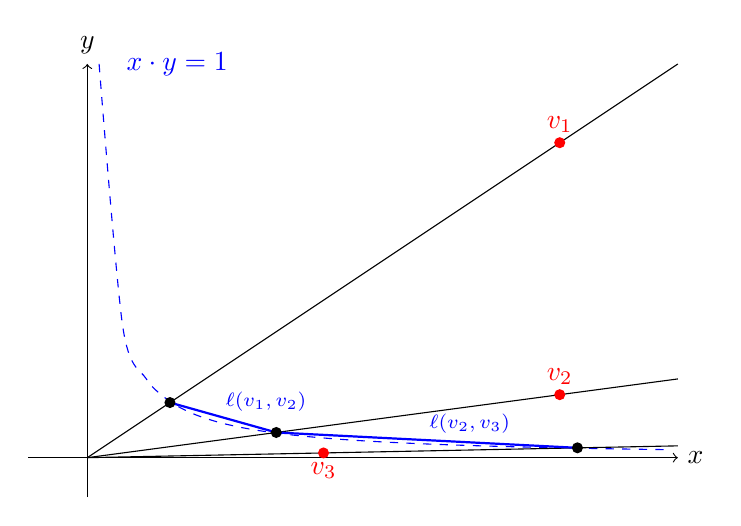
\begin{tikzpicture}[x=1.5cm,y=1cm]
  \draw[->] (-0.5, 0) -- (5, 0) node[right] {$x$};
  \draw[->] (0, -0.5) -- (0, 5) node[above] {$y$};
  \draw[dashed,yscale=0.5, domain=0.1:4.9, smooth, variable=\x, blue] plot ({\x}, {1/\x});
  \node[blue,anchor=west] at (0.25,5) {$x\cdot y=1$};
  \draw[] (0,0) -- (5,5);
  \draw[] (0,0) -- (5,1);
  \draw[] (0,0) -- (5,0.15);
  \coordinate (i1) at (0.7,0.7);
  \coordinate (i2) at (1.6,0.32);
  \coordinate (i3) at (4.15,0.125);
  \coordinate (v1) at (4,4);
  \coordinate (v2) at (4,0.8);
  \coordinate (v3) at (2,0.06);
  \draw[blue,thick] (i1) -- node[anchor=south west,xshift=-1mm,yshift=-0.5mm,font=\scriptsize] {$\ell(v_1,v_2)$} (i2) -- node[anchor=south west,xshift=-1mm,yshift=-0.5mm,font=\scriptsize] {$\ell(v_2,v_3)$} (i3);
  \fill (i1) circle (2pt);
  \fill (i2) circle (2pt);
  \fill (i3) circle (2pt);
  \fill[red] (v1) circle (2pt);
  \fill[red] (v2) circle (2pt);
  \fill[red] (v3) circle (2pt);
  \node[red,above] at (v1) {$v_1$};
  \node[red,above] at (v2) {$v_2$};
  \node[red,below] at (v3) {$v_3$};
  % \draw[scale=0.5, domain=-3:3, smooth, variable=\y, red]  plot ({\y*\y}, {\y});
\end{tikzpicture}
\caption{Example with points v1, v2 and v3}
\end{figure}

In this example, for each point $v_{1}, v_{2}, v_{3}$, they can be represented on the hyperbola and then the distance between these points can be measured using the method we outlined earlier. Note that the distance from $v_{1}$ to $v_{2}$ is, visually, larger than $v_{2}$ to $v_{3}$. However, when measured using the hyperbola, it is clear that the distance of $l(v_{1}, v_{2})$ is smaller than distance of $l(v_{2}, v_{3})$.


\section{Great Circle Distance}
We can also measure distance using circles and geosidics. If we have our start and target point on a circle, we can measure the distance using a geosidic rather than a simple straight line.

However, these geosidic measurements can become unstable and have floating point errors for small distances, since they are based off of the spherical law of cosines. (e.g. $cos(x) \approx 0.999999$ for $x = 0.001$.)

%%Mention something about density of cones?

%%Example of formula

Other formulas that have been conditioned to deal with these small distance floating point errors conversely have problems with antipodal points. Hence we would likely need to implement both formulas, to avoid these errors.

 \begin{thebibliography}{2}
 \bibitem{AndersPHD}
 Anders Jensen.
 \textit{Algorithmic Aspects of Gr\"{o}bner Fans and Tropical Varieties}.
 Aarhus 2007
 \\\texttt{https://math.au.dk/publs?publid=655}
 
 \bibitem{GenericGroebner}
 K. Fukuda, A. N. Jensen, N. Lauritzen, R. Thomas.
 \textit{The generic Groebner walk}
 2005
 \\\texttt{https://arxiv.org/abs/math/0501345v3}
 
 \end{thebibliography}


\end{document}